\documentclass[tikz, border=5, svgnames]{standalone}
\usepackage[utf8]{inputenc}
\usepackage[english]{babel}
\usepackage{amsmath}
\usepackage{amsfonts}
\usepackage{amssymb}
\usetikzlibrary{arrows.meta}
\usepackage{pgfplots}

\begin{document}
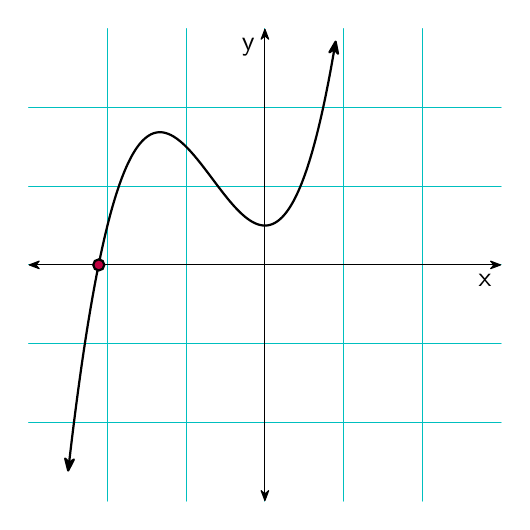
\begin{tikzpicture}

\foreach \i in {-2,...,2}
    \draw[line cap = round, Cyan!75!Black] (\i, -3) -- (\i, 3) %
    (-3, \i) -- (3, \i);

\draw[{Stealth[round]}-{Stealth[round]}] (-3,0) -- (3,0);
\draw[{Stealth[round]}-{Stealth[round]}] (0, -3) -- (0, 3);

\node at (3, 0) [anchor=north east] {$\mathsf{x}$};
\node at (0, 3) [anchor=north east] {$\mathsf{y}$};

\begin{axis}[axis x line=none,axis y line=none,xticklabels=\empty,yticklabels=\empty,xmin=-3, xmax=3,ymin=-3, ymax=3, xshift=-3cm, yshift=-3cm, x=1cm,  y=1cm]

    \addplot [thick, line cap=round, samples=500, domain=-2.5:.90, {Stealth[round]}-{Stealth[round]}] {x^3 + 2*x^2+ 0.5};

\end{axis}

\draw[thick, fill=purple] (-2.11, 0) circle (2pt);

\end{tikzpicture}
\end{document}
